\section{Adapting the Other Passes to Separate Compilation}

In the previous section, we looked at the specific example of constant propagation in detail and
explained how we adapted CompCert's proof of that pass to Level A and B notions of compositional
correctness.  In this section, we discuss some details of other CompCert passes for which adapting
to Level A and B correctness required some interesting (but still not much) work.

\begin{figure*}[t]
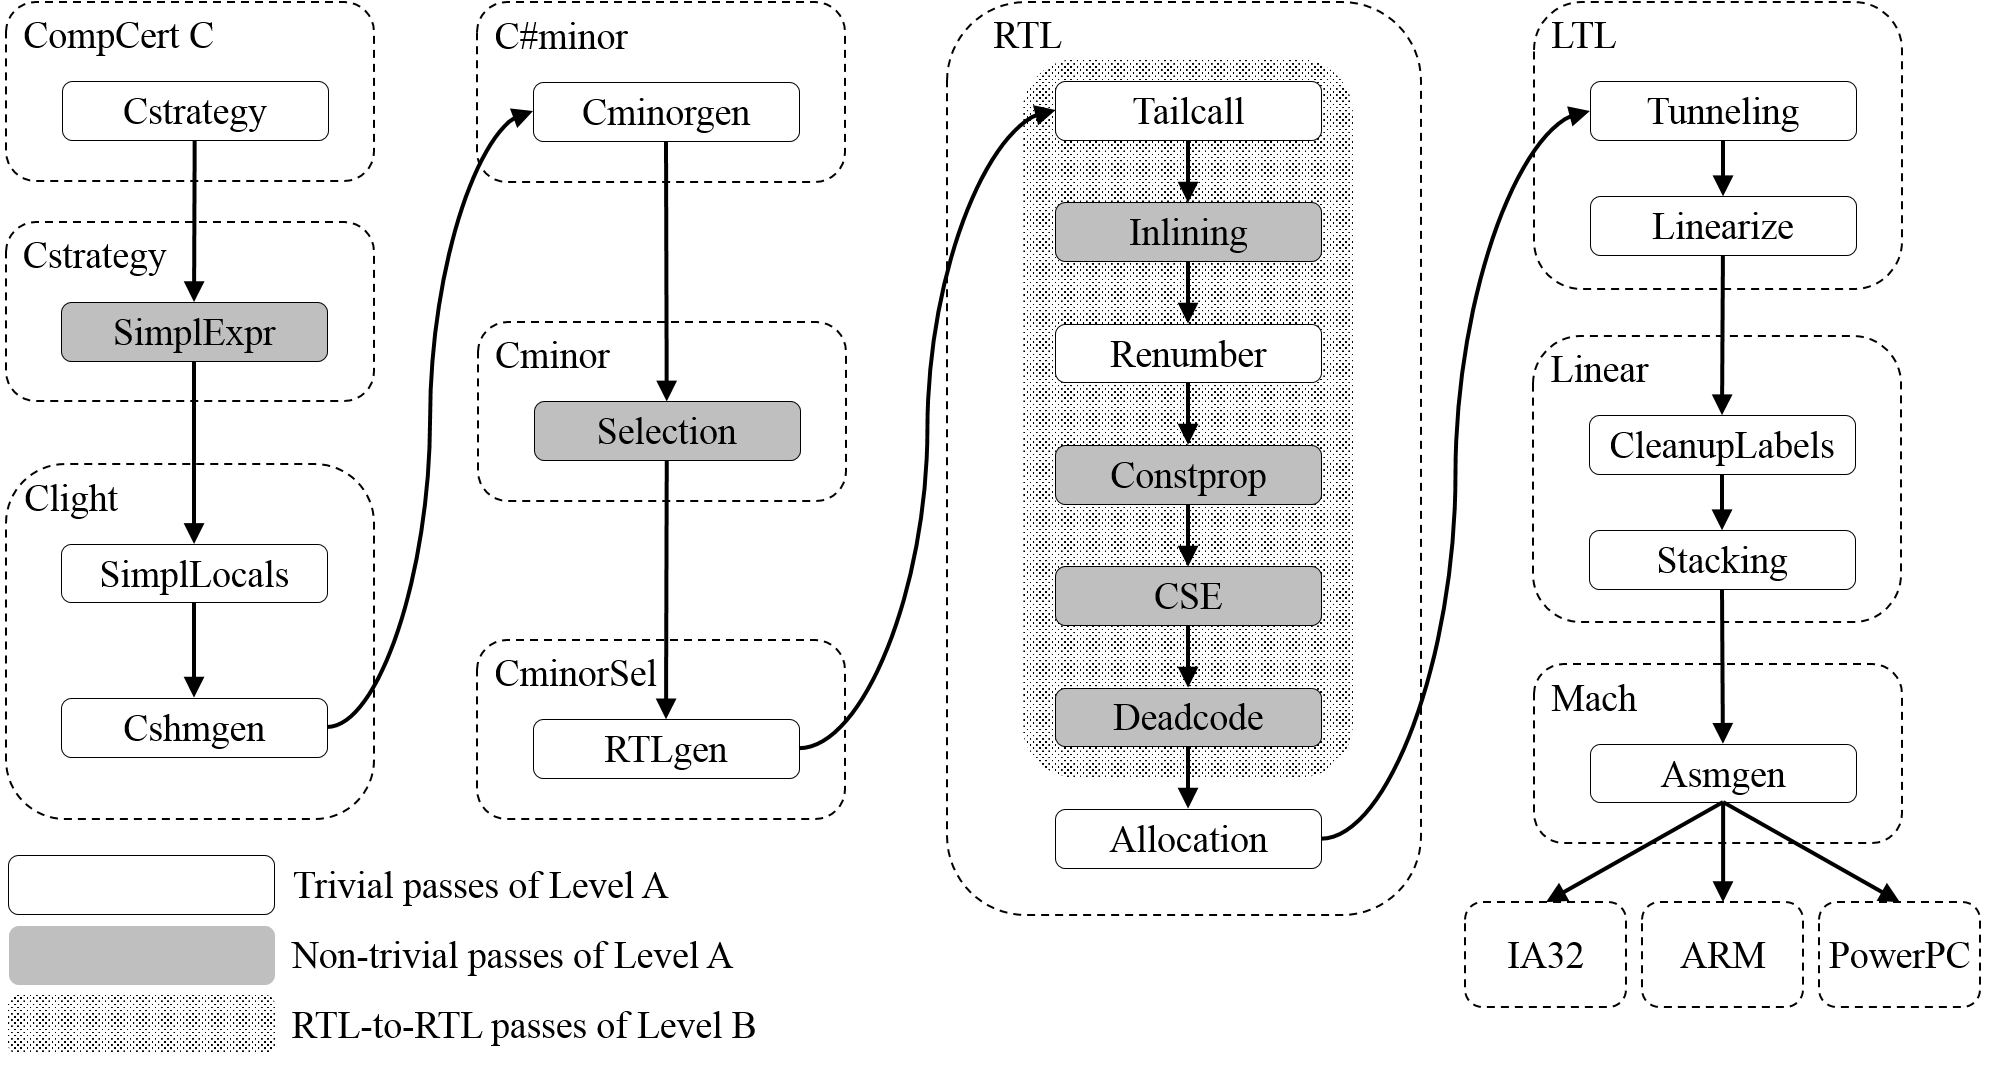
\includegraphics[width=\textwidth]{sepcomp-passes.png}
\caption{Classification of Optimization Passes in CompCert}
\label{fig:sep-comp-passes}
\end{figure*}

\Cref{fig:sep-comp-passes} shows which verification technique we apply to each optimization
pass of CompCert.  For Level A, we apply the trivial technique based on commutativity with linking
to 13 passes and the non-trivial technique to 6 passes.  For Level B, we apply our technique to all
6 RTL-to-RTL passes.

% % Since the trivial
% % case of Level A (when passes commute with linking) is, well, trivial,
% % we do not discuss it here.

% As explained in \Cref{sec:overview:LevelA}, porting 13 of the 19
% passes of CompCert to Level A was trivial because those passes commute
% with syntactic linking.  For porting the remaining passes to Level A,
% and for porting all passes to Level B, we can update the proof, as we
% have seen, in three steps:
% \begin{enumerate}
% \item Update the simulation relation $R$.
% \item Update the proof that $R$ is in fact a simulation relation.
% \item Update the proof that the initial states after loading are
%   related by $R$.
% \end{enumerate}

% \paragraph{CompCert to Level A}

% The general idea for updating the simulation relation is to simply change the
% whole program $\vprg$ to a sub-program $\vsprg$ such that $\vsprg
% \subseteq \vprg$ whenever $\vprg$ is used as compile-time information.
% For example, for the constant propagation pass, we changed
% \[\vfd' = \mathrm{transfun}(\vprg,\vfd)\]
% to
% \[\exists \vsprg \subseteq \vprg.~
% \vfd' = \mathrm{transfun}(\vsprg,\vfd)\] 
% and
% \[
% \soundstate(\vprg,\vprg,s)\]
% to
% \[
% \forall \vsprg \subseteq \vprg.~
% \soundstate(\vprg,\vsprg,s)
% \]
% New proof obligations introduced by these changes essentially amount
% to establishing the monotonicity of various properties: that the
% property continues to hold in a larger program context than was used
% at compilation time.  In CompCert, it turned out that proving such
% monotonicity is quite easy.  We will discuss below what monotonicities
% we had to prove for each optimization in detail.

% \paragraph{Level A to Level B}

% The general idea for updating the simulation relation is to add a case
% to the simulation for when identical functions are invoked in the
% source and target. Here, we can easily derive such invariants as
% special cases from the invariants used in Level A because usual
% optimizations essentially subsume the possibility of nothing being
% optimized.

% New proof obligations introduced by theses updates are essentially
% special cases of existing ones and thus one can easily kill them by
% cut-and-pasting followed by specialization.  More specifically, while
% the original simulation proof shows step-simulation for states where
% only the source and optimized functions are invoked in the current
% state and all stack frames, now we have three more logical cases (\ie
% (current,stack frame) = (optimized,identical), (identical,optimized),
% (identical,identical)). In all RTL-to-RTL passes, we could easily
% adapt existing proofs for the original case (\ie (current,stack frame)
% = (optimized,optimized)) to the other three cases by cutting-and-paste
% and specialization, and thus there is nothing interesting to discuss.

%% However, 

%% the proof of step-simulation for the other three cases
%% ((current,stack frame) = (optimized,identical), (identical,optimized)
%% or (identical,identical)) is almost a special case of the original case
%% ((current,stack frame) = (optimized,optimized)).

%% More specifically,
%% we update the simulation proof as follows:
%% \begin{itemize}
%% \item
%% We first update the existing simulation proof to cover cases where

%% identical functions are 
%% stack frames 

%% when the optmized functions are currently executed.
%% This is easy because stack frames for identical functions are subsumed by
%% those for optmized functions.
%% \item
%% We prove the case where identical functions are currently executed
%% by copy-and-pasting the proof of the case where optimized functios are executed
%% and specializing them.
%% \item 
%% Showing that the initial memories are related is easy by construction.
%% \item
%% Code Refactoring
%% \end{itemize}

%% \todo{jeehoon: moved the descriptions for level B's general pattern
%%   from examples}
%% \begin{itemize}
%% \item match\_fundef : id or translated
%% \item identical case for match\_stacks, match\_identical\_states
%% \item Update lemmas for identical cases by copy-and-pasting.
%% \item Prove the step lemma for identical cases by copy-and-pasting:
%%   $T \to I$, $I \to T$, $ I \to I$ cases.
%% \end{itemize}

\subsection{RTL-Level Optimizations that Rely on Value Analysis}

Three RTL-level optimizations rely on the value analysis: constant propagation, common subexpression
elimination (CSE), and deadcode elimination (DCE).  These passes are inter-procedural solely because
they rely on the value analysis.  Thus, the porting of the proofs of CSE and DCE to support
compositional correctness proceeded analogously to the porting of the constant propagation pass.


\subsection{Selection}

The selection pass ``recognizes opportunities for using combined arithmetic and logical operations
and addressing modes offered by the target processor.''~\cite{compcert-website}.  The pass is mostly
intra-procedural, except for the following two transformations on function calls:

\paragraph{Recognizing Immediate Calls}
The selection pass transforms an indirect call via a function pointer expression, say $e_p$, into an
immediate call, if it can determine that the expression $e_p$ always evaluates to the pointer to an
internal function.  The pass uses a simple analysis $\code{classify\_call}(prg, e_p)$ for
determining this.  For separate compilation, we proved the monotonicity of the analysis: the result
$\code{classify\_call}(sprg, e_p)$ for a subprogram $sprg \subseteq prg$ is sound w.r.t.\ the whole
program $prg$.

\paragraph{64-bit Integer Operations into Library Calls}
The selection pass transforms some 64-bit integer operations into calls to library helper functions.
For example, \code{(long long) f}, a cast from \code{float} to \code{long long}, is transformed into
a call \code{\_\_int64\_dtos(f)} to the corresponding helper function.  For this transformation to
be valid, the pass should ensure that the helper function (\eg \code{\_\_int64\_dtos}) is declared
as an external function in the source program's global environment.  CompCert has a designated
checker $\code{check\_helpers}(prg)$ to ensure this property.

For separate compilation, we proved that the checker for helper functions is monotone
w.r.t. linking: $\code{check\_helpers}(prg1)$ and $\code{check\_helpers}(prg2)$ implies \\
$\code{check\_helpers}(prg1 \circ prg2)$ for all programs $prg1$ and $prg2$.  The proof is a little
bit involved, as linking reorders global declarations, and the corresponding logical blocks for the
helper functions in the global environments may vary.

% Note that the monotonicity we proved for \code{check\_helpers}
% deviates from the general pattern, namely ensuring
% $\code{check\_helpers}(sprg)$ for some $sprg \subseteq prg$.  This
% is because the context $ctx$ of $sprg$, which satisfies
% $sprg \circ ctx = prg$, may redefine library helper functions as
% internal functions, and invalidate the properties on helper functions
% in the whole-program $prg$.

\paragraph{Compiler Bug We Found}
The original CompCert 2.4 used a function $\code{get\_helpers}$
instead of $\code{check\_helpers}$.  We found and reported a
compiler bug related to $\code{get\_helpers}$, which was
subsequently confirmed.
% \footnote{See the README of the supplementary
  % materials for more details.}

We found the bug in the course of proving monotonicity regarding
$\code{get\_helpers}$. This function is directly implemented in
OCaml and its property is axiomatized in Coq as follows:
%\newpage
\begin{minted}{coq}
Axiom get_helpers_correct:
  forall ge hf, get_helpers ge = OK hf ->
  i64_helpers_correct ge hf.
\end{minted}
The problem was that this axiom is not strong enough to prove
monotonicity, and even worse, not true for the OCaml implementation of
$\code{get\_helpers}$. One of the properties this axiom postulates
is that helper functions like \code{\_\_int64\_dtos} are only
declared but not defined in the source program. However,
$\code{get\_helpers}$ does not check it at compile time!

Here is an example that exposes the bug:
\begin{minted}{c}
#include <stdio.h>
long long __i64_dtos(float t) {
  return 3;
}
int main() {
  printf(“%lld\n”, (long long) 5.0f); // expected: 5, actual: 3
  return 0;
}
\end{minted}
Here the cast \code{(long long) 5.0f} is converted to a call to the
library helper function \code{\_\_i64\_dtos(5.0f)} by the selection
pass. However, we successfully hijack the function call by overwriting
the function \code{\_\_i64\_dtos}, which results in printing $3$
instead of the correct result $5$.  Now, strictly speaking, due to the
hijacking of a reserved identifier, this example has undefined
semantics according to the C99 standard, so CompCert's behavior here
is technically legal.  But the dependence on an invalid axiom is
clearly a bug.

After we reported this bug, it was fixed in the development branch of
CompCert (and subsequently CompCert 2.5). In this fix, which we
backported to CompCert 2.4 using \code{git-cherry-pick}, the OCaml
$\code{get\_helpers}$ function is replaced by the aforementioned
$\code{check\_helpers}$, which is implemented and verified directly
in Coq, thereby avoiding the need for an invalid axiom.

\subsection{Inlining}
The inlining pass is inherently inter-procedural, as it replaces a
call to a simple function with the body of the function.  In the pass,
the selector $\code{funenv\_program}(prg)$ chooses internal function
definitions of $prg$ that are worth inlining in other functions.  For
the inlining pass to be valid, the pass should ensure that function
definitions in $\code{funenv\_program}(prg)$ are indeed defined in
the global environment $\rtlgenv(prg)$.

For separate compilation, we proved that the global environment
initialization is monotone for function definitions: if a function
definition, say $fd$, is defined in $\rtlgenv(sprg)$ and $sprg
\subseteq prg$, then $fd$ is also defined in $\rtlgenv(prg)$.  The
proof is a little bit involved for the same reason as for
\code{check\_helpers} in the selection pass: linking reorders global
declarations and the corresponding logical blocks in the global
environments.


\subsection{SimplExpr}
The SimplExpr pass is essentially intra-procedural since just ``side
effects are pulled out of CompCert C expressions''~\cite{compcert-website}.
However, it does not commute with linking because a single counter is
used globally to generate temporary variable names for all function
definitions.

Updating the existing proof was easy because the original simulation
relation $R$ does not bake in the specific way temporary variable
names are generated. Thus, we did not need to change the simulation
relation $R$ and the simulation proof at all.  We just needed to
update the proof that the initial states after loading satisfy the
relation $R$ even in the presence of separate compilation, which
was straightforward.

%% \subsection{TODOs}
%% \begin{itemize}
%% \item explain \code{sepcomp\_rel}
%% \item properties of \code{sepcomp\_rel}
%% \end{itemize}



%%% Local Variables:
%%% mode: latex
%%% TeX-master: "main"
%%% TeX-command-extra-options: "-shell-escape"
%%% End:
